
\documentclass [tikz, border=3mm] {standalone}

%common figure styles
\input{header.htex}


\begin {document}

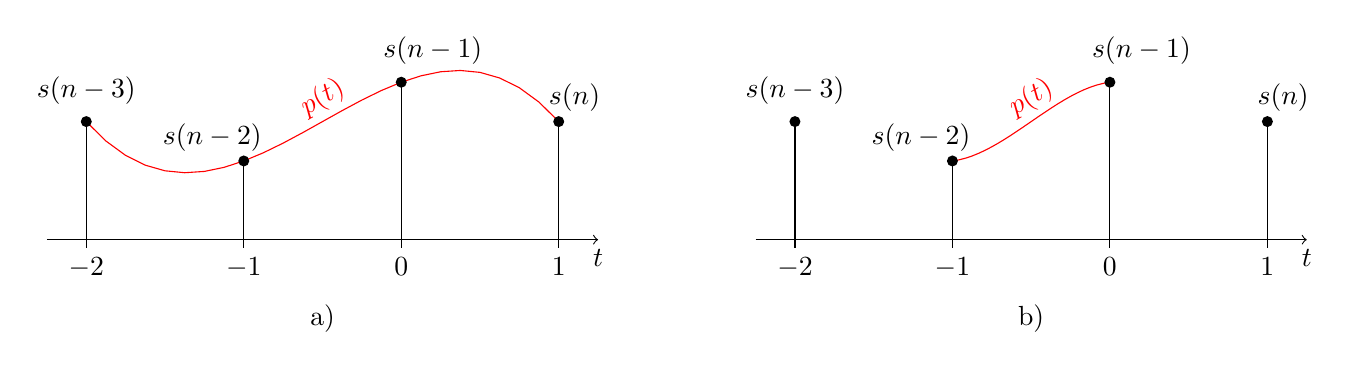
\begin{tikzpicture}

\begin{scope}[xshift = 0cm, yshift = 0cm]
\draw[->] (-0.5cm,	0cm)		-- (6.5cm, 0cm)	node[below] {$t$};

\draw[-, red,  domain = -4.0:2.0, xshift = 4cm] 
plot (\x,  {2+0.75*(\x*0.5)-0.75*(\x*0.5)^2 -0.5*(\x*0.5)^3}) ;

\draw (0, -0.1) node[below]{$-2$} -- (0, 1.5) node[above, yshift = 0.1cm] {$s(n-3)$};
\fill (0, 1.5) circle(0.07cm) ;

\draw (2, -0.1) node[below]{$-1$} --   (2, 1)  node[above, xshift = -0.4cm] {$s(n-2)$};
\fill (2, 1) circle(0.07cm) ;


\draw (4, -0.1) node[below]{$0$}  -- (4, 2)  node[above, xshift = 0.4cm, yshift = 0.1cm] {$s(n-1)$};
\fill (4, 2) circle(0.07cm) ;

\draw (6, -0.1) node[below]{$1$} -- (6, 1.5)  node[above, xshift = 0.2cm] {$s(n)$};
\fill (6, 1.5) circle(0.07cm) ;


\node[red, rotate=30] at (3.0, 1.8) {$p(t)$};
\end{scope}


\begin{scope}[xshift = 9cm, yshift = 0cm]
\draw[->] (-0.5cm,	0cm)		-- (6.5cm, 0cm)	node[below] {$t$};

\draw[-, red,  domain = -2.0:0.0, xshift = 4cm] 
plot (\x,  {2+0.25*(\x*0.5)-2.25*(\x*0.5)^2 -1.5*(\x*0.5)^3}) ;

\draw (0, -0.1) node[below]{$-2$} -- (0, 1.5) node[above, yshift = 0.1cm] {$s(n-3)$};
\fill (0, 1.5) circle(0.07cm) ;

\draw (2, -0.1) node[below]{$-1$} --   (2, 1)  node[above, xshift = -0.4cm] {$s(n-2)$};
\fill (2, 1) circle(0.07cm) ;


\draw (4, -0.1) node[below]{$0$}  -- (4, 2)  node[above, xshift = 0.4cm, yshift = 0.1cm] {$s(n-1)$};
\fill (4, 2) circle(0.07cm) ;

\draw (6, -0.1) node[below]{$1$} -- (6, 1.5)  node[above, xshift = 0.2cm] {$s(n)$};
\fill (6, 1.5) circle(0.07cm) ;


\node[red, rotate=30] at (3.0, 1.8) {$p(t)$};
\end{scope}

\node  at (3, -1) {a)};
\node  at (12, -1) {b)};






 
\end{tikzpicture}

\end {document}
  



